\documentclass[11pt]{amsart}
\usepackage{amsmath,amssymb,amsthm,mathtools,enumitem}
\usepackage[margin=1in]{geometry}
\usepackage{hyperref}
\usepackage{graphicx}

\newtheorem{theorem}{Theorem}[section]
\newtheorem{proposition}[theorem]{Proposition}
\newtheorem{corollary}[theorem]{Corollary}
\theoremstyle{remark}
\newtheorem*{remark}{Remark}

\title{The Cutting Plane: Every Line Through the Multiplication Table Is a Conic Section}
\author{Jeremy Ebert}
\address{Franklin County, Ohio, USA}
\date{2026}

\begin{document}
\maketitle

\begin{abstract}
Write out the ordinary multiplication table and draw a straight line through it. What curve does that line trace, once you plot the factor pairs it passes through in a natural coordinate system built from their sum, difference, and geometric mean? We answer this completely: the type of curve --- ellipse, parabola, or hyperbola --- is fixed by the sign of the line's coefficients, with the familiar circle traced by an anti-diagonal, and the familiar parabolas traced by a single row or column, appearing as two special cases of one proof rather than two separate facts. Along the way, the same coordinate system gives a one-line restatement of Fermat's 1643 factorization method and a short, visual re-derivation of the classical Dirichlet divisor summatory function.
\end{abstract}

\section{Introduction}

Figure~\ref{fig:table_line}(b) shows the ordinary multiplication table itself, not a stand-in for it: every small square is one product $xy$, sitting where its row and column cross, filled in out to the anti-diagonal $x+y=12$. It is drawn in the $(X,T)$ coordinates of Section~2 rather than the usual $(x,y)$ grid, which is why it comes out as a triangle rather than a square --- but the entries, and what they mean, are exactly the ordinary table. A single dashed line, $x+y=8$, runs across it, passing through three of those squares: the cells $(2,6)$, $(4,4)$, $(6,2)$, holding $12$, $16$, $12$. That is what we mean by ``a line through the multiplication table'': a line drawn across this arrangement of squares, passing through some of them and not others.

Take the one cell $(2,6)$, area $12$. There is a classical construction --- known to Euclid --- for turning any rectangle into a square of the same area: lay the rectangle's two sides, $2$ and $6$, end to end as the diameter of a semicircle, and erect a perpendicular at the point where they join. That perpendicular, from the diameter up to the semicircle, has length exactly $\sqrt{12}$ --- the side of a square with the same area as the $2$-by-$6$ rectangle it came from. This is the right-triangle altitude theorem, and it hands us three numbers straight from the construction: the semicircle's radius, $T=(x+y)/2=4$; the altitude itself, $Y=\sqrt{xy}=\sqrt{12}$; and the signed distance $X=(x-y)/2=-2$ from the semicircle's center to the foot of the altitude. Pythagoras, applied to the right triangle formed by the center, the foot of the altitude, and the top of the altitude, gives
\[
X^2+Y^2=T^2
\]
immediately --- no algebra required, just the construction. (Expanding $\left(\frac{x-y}2\right)^2+xy=\left(\frac{x+y}2\right)^2$ confirms it symbolically, but the semicircle is why it is true.) For cell $(2,6)$: $4+12=16$, exactly $T^2$.

So every square in Figure~\ref{fig:table_line}(b) is secretly a point on the cone $X^2+Y^2=T^2$ in three dimensions, and the question that opened this note follows immediately: the three cells on $x+y=8$ all share the same radius $T=4$, so all three land on the same circle --- shown in panel (a), and traced out as an actual circle on the cone in panel (c). What about a line that is \emph{not} an anti-diagonal --- a line like $8x+4y=32$, which does not hold $x+y$ fixed at all? Figure~\ref{fig:table_line} carries this line, together with its mirror image $4x+8y=32$ (the same line with $x$ and $y$ swapped), through the full construction, three ways: flattened onto a plane of circles, in the triangular table itself, and as an actual plane slicing the cone in three dimensions --- which is where the title of this note comes from. The two ellipses are exact reflections of each other across $X=0$, and each one's low end lands exactly on the radius of the $x+y=8$ circle already in view. Section~2 sets up the coordinate system properly; Section~3 answers the general question for an arbitrary line and proves it completely; Sections~4 and~5 show what the same coordinate system buys classically, recovering Fermat's factorization method and the Dirichlet divisor summatory function as direct consequences of the same rows, hyperbola, and diagonal already on the page.

\begin{figure}[h]
\centering
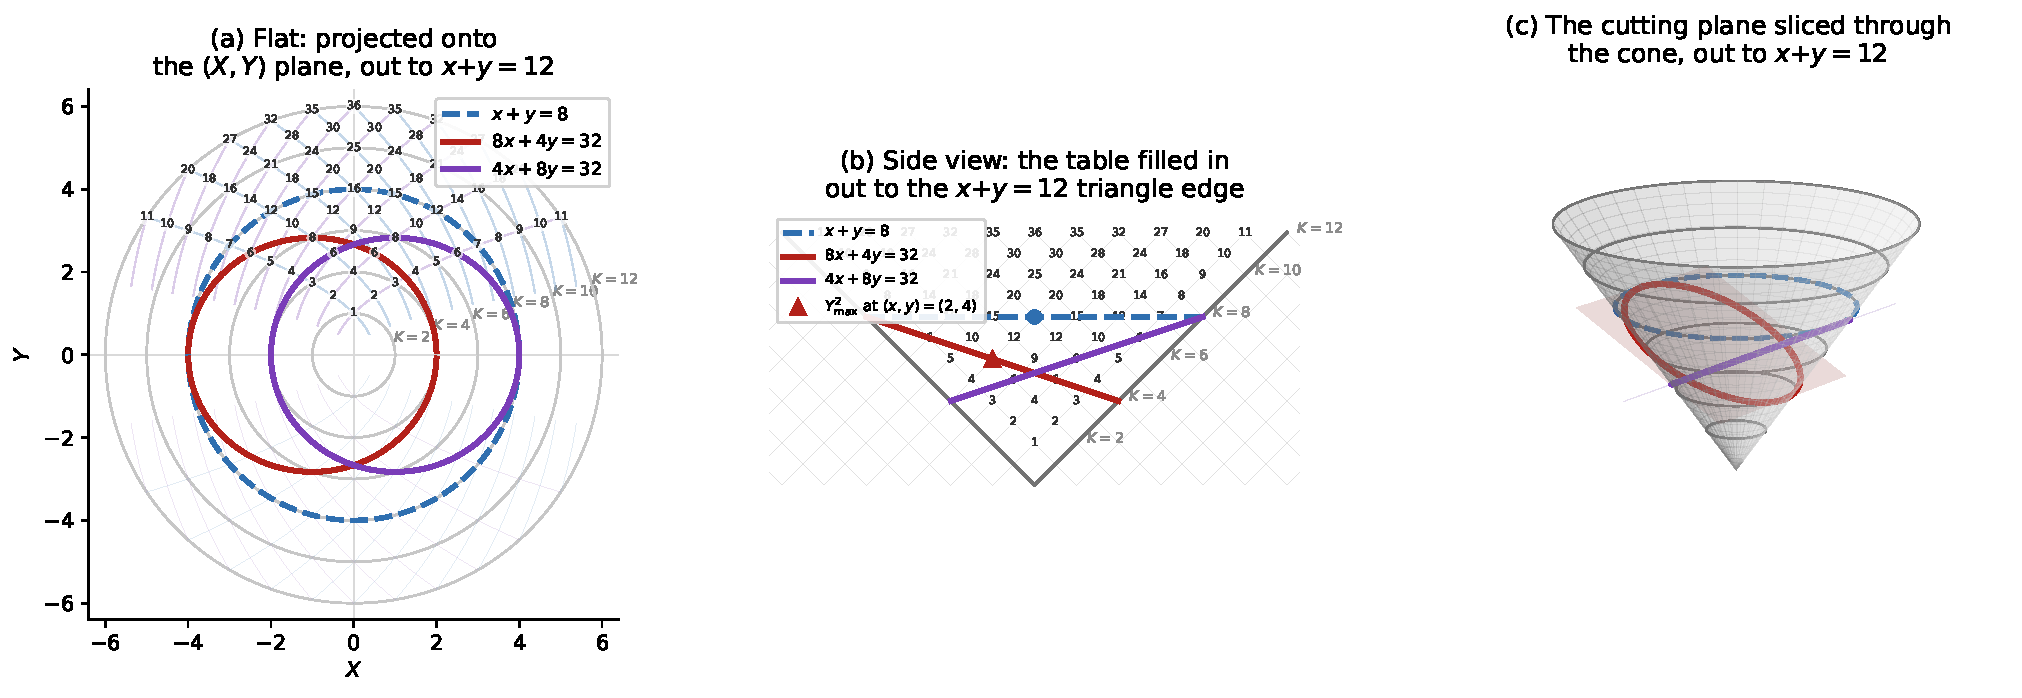
\includegraphics[width=\textwidth]{fig_cutting_plane_3panel.pdf}
\caption{The anti-diagonal $x+y=8$ together with the ellipse $8x+4y=32$ (red) and its mirror image $4x+8y=32$ (purple, the same line with $x$ and $y$ swapped), shown three ways, with the whole multiplication table filled in out to the anti-diagonal $x+y=12$. (a) Projected onto the flat $(X,Y)$ plane: the concentric grey circles are the anti-diagonal circles $X^2+Y^2=T^2$ at fixed $T$, one for each even $K=x+y$ from $2$ to $12$ --- each circle's own diameter is exactly $K$; the faint blue and purple curves are the two mirror-image parabola families of Theorem~\ref{thm:conic}(b) --- rows (fixed $x$) and columns (fixed $y$). The anti-diagonal $x+y=8$ (dashed blue) is exactly the $T=4$ circle; the two ellipses are exact reflections of each other across $X=0$, and each one touches that circle's own radius at its low end ($X=-4$ for the red ellipse, $X=+4$ for its purple mirror). (b) The multiplication table itself, in the $(X,T)$ side view of Section~2: every square is one product $xy$, and the dashed line $x+y=8$ runs directly through three of them --- $(2,6),(4,4),(6,2)$, holding $12,16,12$. The anti-diagonal projects to the full horizontal segment $T=4$, $X\in[-4,4]$, since $T$ is fixed at $4$ while $X=(x-y)/2$ still ranges over every split of $8$, while each ellipse becomes a straight cutting line $(a-b)X+(a+b)T=c$ seen edge-on, the two lines crossing near the table's center. (c) Both cutting planes sliced through the cone $X^2+Y^2=T^2$ in three dimensions: each meets the cone in one of the two ellipses of Theorem~\ref{thm:conic}, traced in red and purple, alongside the anti-diagonal's circle (blue, dashed) for comparison.}
\label{fig:table_line}
\end{figure}

\section{Mean-Value Coordinates and the Conic Identity}

For a factor pair $(x,y)$ with $x,y>0$, define
\begin{equation}
X=\frac{x-y}2,\qquad Y=\sqrt{xy},\qquad T=\frac{x+y}2. \tag{2.1}
\end{equation}
These satisfy the AM--GM identity
\begin{equation}
X^2+Y^2=T^2. \tag{2.2}
\end{equation}
Fixing the anti-diagonal $x+y=K$ fixes $T=K/2$, so (2.2) restricts to the circle $X^2+Y^2=(K/2)^2$: a circle of radius $T=K/2$, so $K$ itself is nothing but that circle's diameter. As $x$ ranges over $1,\dots,K-1$ with $y=K-x$, the point $(X,Y)$ traces $K-1$ discrete points on that circle, with the diagonal point $x=y=K/2$ (when $K$ is even) sitting at the apex $X=0$, $Y=K/2$. Stacking these circles as $K$ varies produces the double-napped cone $X^2+Y^2=T^2$ in $(X,Y,T)$-space; this is the coordinate system used throughout.

\begin{remark}
Although $Y^2=xy$ recovers a cell's flat area as a single number, the map $(x,y)\mapsto(X,Y,T)$ that places that cell on the cone is not area-preserving: the patch of the cone's surface a fixed table cell actually occupies varies with position, smallest near the diagonal $x=y$ and growing without bound as a cell moves off it. We do not need this fact here, and record the exact distortion factor, together with an independent cross-check of it, in a companion note \cite{Ebert2026Area}.
\end{remark}

\section{The General Conic Theorem}

The anti-diagonal $x+y=K$ is one line through the multiplication table among infinitely many. This section answers the natural question completely: what does an arbitrary line $ax+by=c$ produce?

\begin{theorem}\label{thm:conic}
Let $a,b$ be real numbers, not both zero, and $c$ a real number, and consider the line $ax+by=c$ intersecting the multiplication table. On the cone $X^2+Y^2=T^2$, this line traces:
\begin{itemize}
\item an ellipse if $ab>0$, with the circle of Section~2 as the symmetric special case $a=b$;
\item a parabola if $ab=0$ --- the rows ($b=0$) and columns ($a=0$) of the table;
\item a hyperbola if $ab<0$ --- a family distinct from the constant-product hyperbolas of Section~4.
\end{itemize}
\end{theorem}

\begin{proof}
For $b\ne0$, solve $ax+by=c$ for $y=(c-ax)/b$ and substitute into $Y^2=xy$:
\begin{equation}
Y^2=\frac cb x-\frac ab x^2, \tag{3.1}
\end{equation}
a quadratic function of $x$ with leading coefficient $-a/b$. When $ab>0$ this coefficient is negative, so $Y^2$ rises from $0$, reaches a maximum, and returns to $0$ as $x$ ranges over its real domain: a bounded, non-degenerate real conic is an ellipse. The case $a=b$ is the anti-diagonal $x+y=c/a$, whose ellipse degenerates by symmetry to the circle of Section~2. When $ab<0$ the coefficient is positive, so $Y^2$ grows without bound: an unbounded hyperbola. The case $b=0$ (or $a=0$) is a row or column, treated next.
\end{proof}

\begin{proposition}[Rows and columns are parabolas]
For a row $x=c$, $X+T=c$ and $Y^2=c(T-X)$; for a column $y=c$, $T-X=c$ and $Y^2=c(X+T)$. Both are parabolas.
\end{proposition}

\begin{proof}
Substituting $x=c$ into $X=(x-y)/2$, $T=(x+y)/2$ gives $X+T=c$ identically, independent of $y$; writing $W=T-X$, we get $W=y$, so $Y^2=xy=cW$. This is the classical construction of a parabola as a conic section: the plane $X+T=c$ has normal vector $(1,0,1)$, and the cone has a generator direction $(-1,0,1)$ lying on it, since $(-1)^2+0^2=1^2$. Since $(1,0,1)\cdot(-1,0,1)=0$, the plane $X+T=c$ is parallel to that generator --- and slicing a cone with a plane parallel to (but not through) one of its own generators is exactly the classical definition of a parabola. Columns use the mirror generator $(1,0,1)$, by the same argument with $T-X=c$.
\end{proof}

Concretely: the row $x=1$ ($y=1,2,3,4,\dots$) satisfies $X+T=1$ throughout, with $Y^2=y$ taking the values $1,2,3,4,\dots$; the row $x=2$ satisfies $X+T=2$, with $Y^2=2y$ taking the values $2,4,6,8,\dots$; and so on for every row.

\begin{proposition}[Semi-axes and eccentricity, ellipse case]\label{prop:semiaxes}
For $ab>0$, $Y^2$ is maximized exactly at $x=c/(2a)$, where it equals $c^2/(4ab)$ --- and this maximum sits at the midpoint of the line's two axis intercepts, $(c/a,0)$ and $(0,c/b)$.
\end{proposition}

\begin{proof}
Differentiating (3.1) and setting the result to zero gives $x=c/(2a)$; substituting back gives $Y^2_{\max}=c^2/(4ab)$. The intercepts are $x=c/a$ (at $y=0$) and $x=0$ (at $y=c/b$), whose midpoint in $x$ is $c/(2a)$.
\end{proof}

For the line $8x+4y=32$ of Figure~\ref{fig:table_line} ($a=8,b=4,c=32$), this predicts the maximum at $(x,y)=(2,4)$, with $Y^2_{\max}=1024/128=8$, matching $xy=2\cdot4=8$ exactly and matching the marked point in Figure~\ref{fig:table_line}(b). Its mirror image $4x+8y=32$ (swap $a$ and $b$) has the same maximum value $Y^2_{\max}=8$ at the reflected point $(x,y)=(4,2)$, by the symmetry of the formula under $a\leftrightarrow b$.

Proposition~\ref{prop:semiaxes} locates the ellipse's coordinate maximum $Y_{\max}$, but says nothing yet about the ellipse's actual shape as a curve in three-dimensional space --- its true semi-axes, eccentricity, and circumference, as opposed to a single coordinate extremum. These follow from the same symmetry already built into the construction.

\begin{proposition}[True semi-axes, eccentricity, and circumference]\label{prop:trueaxes}
For $ab>0$, the ellipse traced by $ax+by=c$ on the cone has semi-minor axis $b_{\rm semi}=Y_{\max}=c/(2\sqrt{ab})$, semi-major axis
\[
a_{\rm semi}=\frac{c\sqrt{2(a^2+b^2)}}{4ab},
\]
eccentricity
\[
e=\frac{|a-b|}{\sqrt{a^2+b^2}},
\]
depending only on the ratio $a/b$ and not on $c$, and circumference $C=4a_{\rm semi}E(e)$, where $E$ is the complete elliptic integral of the second kind.
\end{proposition}

\begin{proof}
The curve is symmetric under $Y\mapsto-Y$, since $Y=\sqrt{xy}\ge0$ by convention but the underlying identity $Y^2=xy$ is manifestly even in $Y$; a genuine ellipse has at most two axes of symmetry, so $Y=0$ and the pure-$Y$ direction through the ellipse's center must be exactly its two principal axes. The pure-$Y$ direction meets the curve at $Y=\pm Y_{\max}$ (Proposition~\ref{prop:semiaxes}), giving semi-minor axis $b_{\rm semi}=Y_{\max}=c/(2\sqrt{ab})$. The line $Y=0$ meets the curve at exactly its two intercepts, $x=0$ (so $X=-c/(2b)$, $T=c/(2b)$) and $x=c/a$ (so $X=c/(2a)$, $T=c/(2a)$); the distance between these two points is the full major axis, and squaring and simplifying gives $(2a_{\rm semi})^2=\tfrac{c^2}2\big(\tfrac1{a^2}+\tfrac1{b^2}\big)$, i.e.\ the stated $a_{\rm semi}$. Eccentricity follows from $e^2=1-b_{\rm semi}^2/a_{\rm semi}^2$, which simplifies to $(a-b)^2/(a^2+b^2)$ after substitution. Circumference is the standard formula for an ellipse of semi-major axis $a_{\rm semi}$ and eccentricity $e$. All of this was verified independently by direct numerical arc-length integration of the space curve $(X(x),Y(x),T(x))$, agreeing with $4a_{\rm semi}E(e)$ to six decimal places on several unrelated choices of $a,b,c$, including this section's own worked example: for $8x+4y=32$, $a_{\rm semi}=\sqrt{10}$, $b_{\rm semi}=2\sqrt2$, $e=1/\sqrt5$, and $C\approx18.83497$.
\end{proof}

Since $e=0$ exactly when $a=b$, the anti-diagonal's own circle is recovered as the eccentricity-zero special case of Proposition~\ref{prop:trueaxes}, consistent with Theorem~\ref{thm:conic}.

The case $ab<0$ --- a line like $x-y=d$, a fixed difference rather than a fixed sum --- produces a hyperbola by the same mechanism run in reverse: the coefficient $-a/b$ in (3.1) is positive, so $Y^2$ grows without bound. This is a genuinely different construction from the constant-product hyperbolas of Section~4, arising from a linear rather than a multiplicative condition; we do not develop it further here beyond noting that Theorem~\ref{thm:conic} places the ellipse, the parabola, and this second hyperbola family under one proof.

\begin{remark}
Theorem~\ref{thm:conic} is itself a special case of the classical fact that any plane section of a quadric surface is a conic section; what it contributes is the explicit classification, by the sign of $ab$, for the specific family of planes that lines through the multiplication table happen to produce.
\end{remark}

\section{Constant-Product Curves and Fermat's Factorization Method}

A different, non-linear curve family fixes the product rather than a linear combination: $xy=N$. Since $Y^2=xy$, this fixes $Y^2=N$ in (2.2), giving
\begin{equation}
T^2-X^2=N. \tag{4.1}
\end{equation}
This is exactly Fermat's factorization method (1643): to factor an odd $N$, test successive integers $a\ge\lceil\sqrt N\rceil$ until $a^2-N$ is a perfect square $b^2$, at which point $N=a^2-b^2=(a-b)(a+b)$ is a factorization. The search terminates fastest when $N$ has a factor pair close to $\sqrt N$, i.e.\ when the corresponding $X$ is small. In the coordinates of Section~2, $a=T$ and $b=X$ exactly, so the constant-product curve $xy=N$ is the graph of every factorization Fermat's method could find, and (4.1) is simply that method's defining equation, restated three and a half centuries later in mean-value coordinates.

\section{The Divisor Summatory Function via Nested Gnomons}

The coordinate system of Sections~2--4 also gives a short, visual re-derivation of a classical object: the divisor summatory function $D(n)=\sum_{k=1}^nd(k)$, the number of lattice points $(x,y)$ with $x,y\ge1$ and $xy\le n$. Dirichlet's 1849 hyperbola method sums full rows or columns and removes the double-counted square of side $\lfloor\sqrt n\rfloor$. Here we anchor the same count on the diagonal $x=y$ instead --- the spine from which the circles of Section~2 radiate.

For each vertex $(u,u)$ with $1\le u\le\lfloor\sqrt n\rfloor$, form the L-shaped gnomon consisting of the vertex itself, a horizontal arm along $y=u$ out to the hyperbola at $x=\lfloor n/u\rfloor$ (containing $\lfloor n/u\rfloor-u$ points), and, by the symmetry of the region under $x\leftrightarrow y$, an identical vertical arm. This is not a new object: the horizontal arm is the row $y=u$, the very parabola $Y^2=u(X+T)$ of Proposition~3.2, and the point where the gnomon's arm stops is exactly where that row meets the constant-product hyperbola $xy=n$ of Section~4. Writing the row as $x=n/u$ at that crossing, the arm's length is
\[
\frac nu-u,
\]
a continuous quantity measured along a curve already on the page; the only new ingredient is capping it at an integer lattice point, which is where the floor function in $\lfloor n/u\rfloor-u$ comes from. So each gnomon arm is a specific, finite piece of a row-parabola, cut off by the constant-product hyperbola and then discretized --- the same two curve families from Sections~3 and~4, run out from the diagonal spine of Section~2 until they hit each other. The total count is
\begin{equation}
D(n)=\sum_{u=1}^{\lfloor\sqrt n\rfloor}\left[2\left\lfloor\frac{n-u^2}u\right\rfloor+1\right]. \tag{5.1}
\end{equation}
Expanding algebraically --- using $u^2/u=u$ to pull $u$ out of the floor function, then applying $\sum u=k(k+1)/2$ with $k=\lfloor\sqrt n\rfloor$ --- collapses this to
\begin{equation}
D(n)=2\sum_{u=1}^{\lfloor\sqrt n\rfloor}\left\lfloor\frac nu\right\rfloor-\lfloor\sqrt n\rfloor^2, \tag{5.2}
\end{equation}
exactly the textbook symmetric form of the Dirichlet hyperbola identity. The formula itself is of course not new; what is worth noting is that it did not have to be imported --- it is generated in place by objects Sections~2--4 already built: the diagonal spine that anchors the circles, the row-parabolas of Theorem~\ref{thm:conic}, and the constant-product hyperbola of Section~4, with a single floor function marking the one place a continuous crossing height becomes a discrete lattice count.

\section{Discussion}

Sections~2--5 rest on one piece of elementary algebra, the AM--GM identity $X^2+Y^2=T^2$, and one classification theorem built on top of it: every line through the multiplication table produces a conic on the resulting cone, its type fixed by the sign of $ab$ (Theorem~\ref{thm:conic}). Circles and the row/column parabolas are now special cases of a single proof rather than two separate facts, and a genuine ellipse family comes along for free. Section~4 identifies the constant-product hyperbolas with Fermat's 1643 factorization method, and Section~5 shows the same coordinate system reorganizing the classical divisor summatory function around its own diagonal spine. The throughline is a single mechanism, stated once and used three times: every curve considered here is what results from intersecting a plane or a hyperbola with the quadric surface that $Y=\sqrt{xy}$ generates by definition.

\begin{thebibliography}{9}
\bibitem{Dickson} L.~E.~Dickson, \emph{History of the Theory of Numbers, Vol.~I}, Carnegie Institution, 1919, Ch.~14.
\bibitem{Dirichlet} P.~G.~L.~Dirichlet, \"Uber die Bestimmung der mittleren Werthe in der Zahlentheorie, \emph{Abh.\ K\"onigl.\ Preuss.\ Akad.\ Wiss.} (1849), 69--83.
\bibitem{Ebert2026Area} J.~Ebert, \emph{A Semiclassical Band-Area Correspondence for the AM--GM Cone}, Preprint (2026).
\end{thebibliography}

\end{document}
